\documentclass{standalone}
\usepackage{ tikz }
\usetikzlibrary{shapes}
\usetikzlibrary{plotmarks}
\usepackage{ xparse }
\usepackage{../../../macros}

\begin{document}
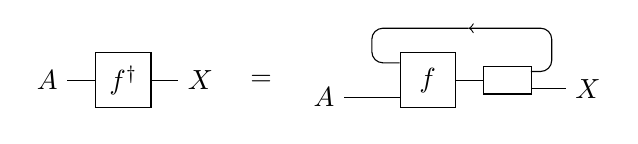
\begin{tikzpicture}[yscale=-1,x=1em,y=1.25em]
    
    \node [anchor=east] at (-11,-0.5) {$A$};
    \draw (-11,-0.5) -- (-10,-0.5);
    \node[draw, minimum height = 2em, minimum width = 2em, anchor = west] at (-10,-0.5){$f^\dagger$};
    \draw (-8,-0.5) -- (-7,-0.5);
    \node [anchor=west] at (-7,-0.5) {$X$};

    \node at (-4,-0.5) {$=$};

    \node [anchor=east] at (-1,0) {$A$};
    \draw (-1,0) -- (1,0);
    \node[draw, minimum height = 2em, minimum width = 2em, anchor = west] at (1,-0.5){$f$};
    \draw (3,-0.5) -- (4,-0.5);
    \node[draw, minimum height = 1em, minimum width = 1.75em, anchor = west] at (4,-0.5){$\ccopy{}$};
    \draw [rounded corners, ->] (5.75,-0.75) -- (6.5,-0.75) -- (6.5, -2) -- (3.5, -2);
    \draw [rounded corners] (3.5,-2) -- (0,-2) -- (0,-1) -- (1,-1);
    \draw [rounded corners] (5.75, -0.25) -- (7,-0.25);
    \node [anchor=west] at (7,-0.25) {$X$};

\end{tikzpicture}
\end{document}